\documentclass{suturo}

\begin{document}
    \maketitle{Motion}{29.12.2017}{}{1}{}{}{}{}

\makeatletter
\newcommand{\chapterauthor}[1]{%
  {\parindent0pt\vspace*{-27pt}%
  \linespread{0}\small\begin{flushright}von: #1\end{flushright}%
  \par\nobreak\vspace*{0pt}}
  \@afterheading%
}
\makeatother

\section{Node: main (motion\_suturo\_1718)}
\subsection{Architekturbild}
\chapterauthor{Roman Haak}
\begin{center} 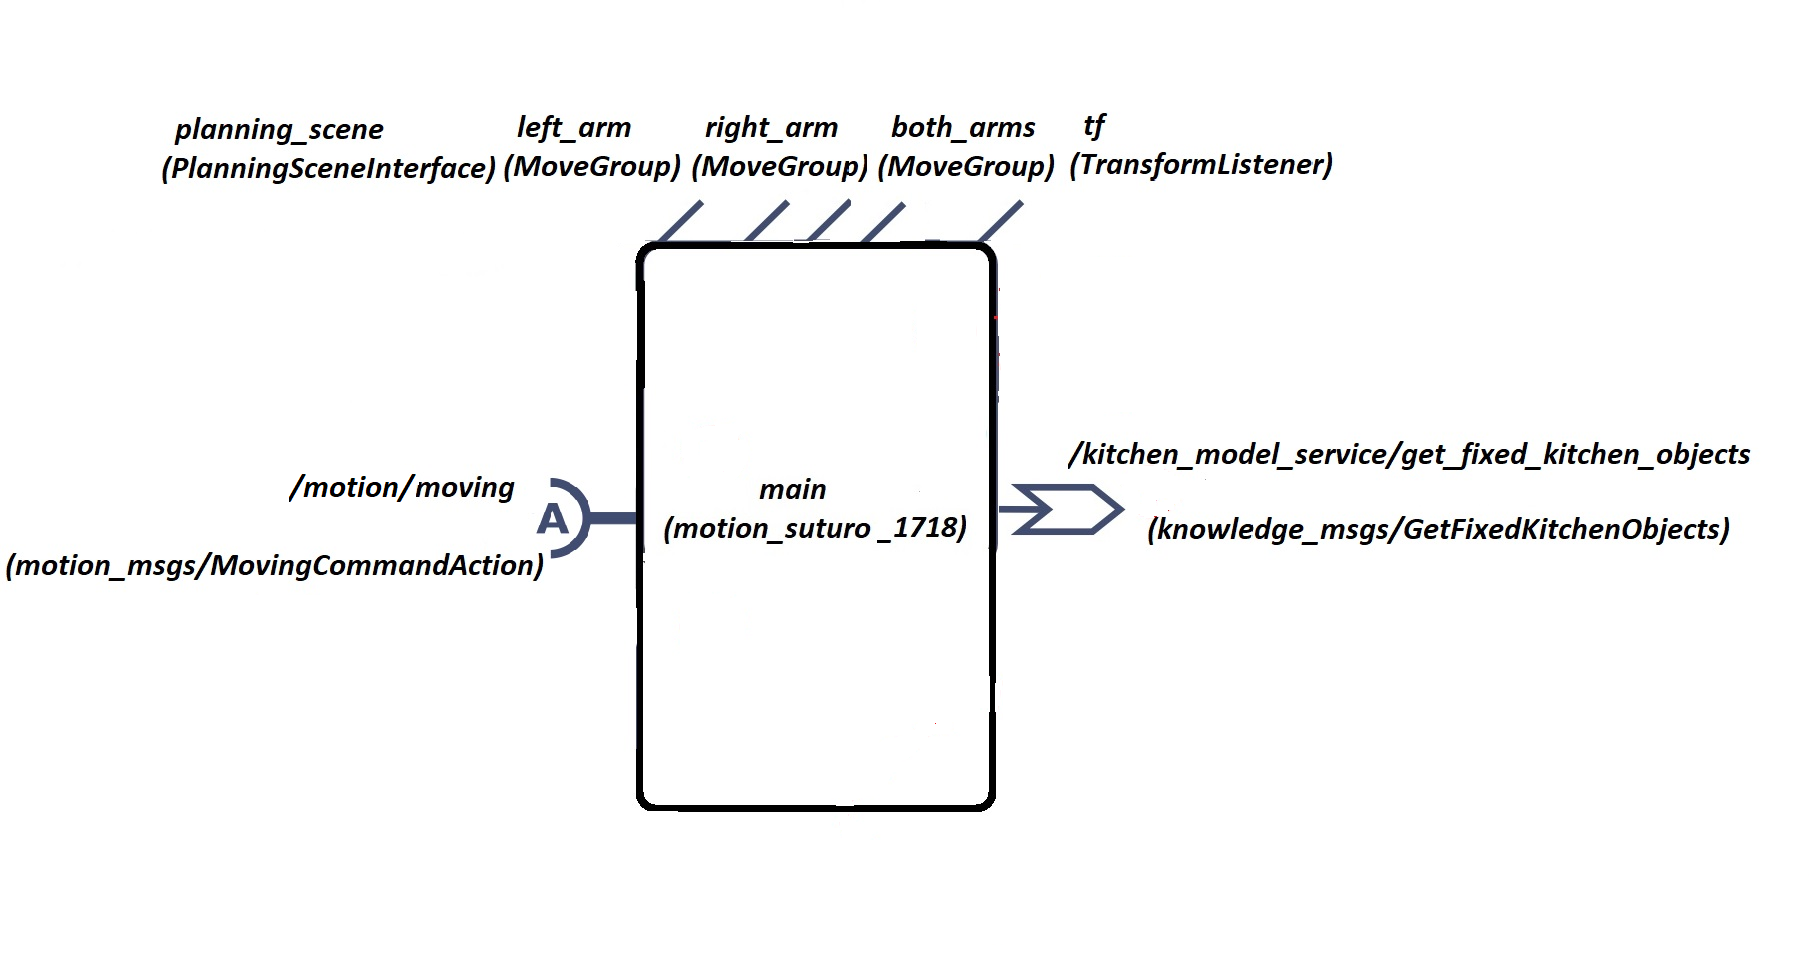
\includegraphics[width=0.8\textwidth]{img/Architekturbild.png} \end{center}

\subsection{API}
\subsubsection{Übersicht}
\chapterauthor{Roman Haak}
Dieser Teil des Systems ist für das Bewegen des PR2 in eine bestimmte Position, bzw. zu einem bestimmten Punkt hin verantwortlich.\\
Zum Ausführen von Bewegungen des PR2 benutzen wir das '\textit{MoveIt-Framework}'. Dieses Framework bietet dabei ein '\textit{MoveGroup-Interface}' an, mit dessen Hilfe es dem Benutzer möglich ist, mit einfachen Funktionsaufrufen Bewegungen auszuführen. Die dahinter steckenden Logiken und Umrechnungen, welche zum letztendlichen Bewegen des Armes nötig sind, werden dann von dem Framework umgesetzt, ohne dass der Benutzer sich darum kümmern muss.\\
Wie wir dieses Framework benutzen, wird im Folgenden vorgestellt.

\subsubsection{Klassenvariablen}
\chapterauthor{Roman Haak}
Im Folgenden werden kurz die wichtigsten Variablen der Klasse '\textit{main}' vorgestellt, um die Funktionsweise des \textit{MoveGrop-Interfaces} zu verdeutlichen:\\\\
\textit{\textbf{planning\_scene}} vom Typ \textit{\textbf{PlanningSceneInterface}}:\\
Über diese Variable ist es uns möglich die sogenannte '\textit{PlanningScene}' des PR2 zu befüllen. Über die \textit{PlanningScene} wird dem PR2 signalisiert, an welcher Stelle sich Objekte befinden, damit Kollisionen mit diesen Vermieden werden können. Wird von dem Benutzer versucht, über das \textit{MoveIt\_Framework} eine Bewegung auszuführen, prüft das Framework zunächst, ob diese Bewegung kollisionsfrei ausgeführt werden kann und bricht mit entsprechender Fehlermeldung ab, falls es in der \textit{PlanningScene} ein Objekt gibt, mit dem der PR2 kollidieren würde. \\
Die Objekte der PlanningScene sind in unserem Fall die Küchenobjekte der IAI-Küche und werden definiert durch einen '\textit{Box-Collider}' mit gewisser Höhe, Breite und Länge.\\\\
\textit{\textbf{both\_arms}}, \textit{\textbf{left\_arm}}, \textit{\textbf{right\_arm}} vom Typ \textit{\textbf{MoveGroupInterface}}:\\
Über Variablen des \textit{MoveGroupInterfaces} können Befehle zum Bewegen eines bestimmten Körperteils abgeschickt werden. Bei uns gibt es dabei drei Gruppen für linken, rechten und beide Arme.\\
So können wir den Endpunkt der jeweiligen kinematischen Kette zu einem bestimmten Punkt hinbewegen oder auch die Gelenkwinkel der Gelenke einer Gruppe einstellen. Das Berechnen einer Trajektorie übernimmt dabei das \textit{MoveIt-Framework}.\\
Es wird von dem \textit{MoveGroup}-Objekt eine entsprechende Rückmeldung in Form eines \textit{MoveItErrorCodes} über den Erfolg der Ausführung gegeben.\\\\
\textit{\textbf{tf}} vom Typ \textit{\textbf{TransformListener}}:\\
Mit Hilfe des \textit{TransformListeners} können Transformationen zwischen Koordinatensystemen zu einem bestimmten Zeitpunkt durchgeführt werden. Das ist in unserem Fall z.B. nötig, wenn der Arm zu einem bestimmten Punkt bewegt werden soll, der aber in einem anderen Koordinatensystem angegeben ist, als unser \textit{MoveGroup}-Objekt zum Planen verwendet.\\

\subsubsection{Serviceclient}
\chapterauthor{Roman Haak}
'\textit{/kitchen\_model\_service/get\_fixed\_kitchen\_objects}': \\
Dieser Service wird beim Initialisieren unseres Programms aufgerufen. Hierüber werden die Abmessungen der Objekte der IAI-Küche in die \textit{PlanningScene} geladen, damit der Roboter sich nur kollisionsfrei bewegt(siehe \textit{Kapitel 1.2.2}, Abschnitt zur '\textit{planning\_scene}').\\
Die Objekte sind dabei durch eine Höhe, Breite und Länge als \textit{Box-Collider} definiert.


\subsubsection{ActionServer}
\chapterauthor{Maximilian Bertram}
'\textit{/motion/moving}': \\
Vom Typ '\textit{motion\_msgs/MovingCommand}': \\
\begin{lstlisting}
#goal definition
geometry_msgs/PointStamped point_stamped
uint8 command
uint8 UNKNOWN=0
uint8 MOVE_STANDARD_POSE=1
uint8 MOVE_RIGHT_ARM=2
uint8 MOVE_LEFT_ARM=3
---
#result definition
bool successful
---
#feedback definition
#bool finished
\end{lstlisting}
\newpage
Über die MovingCommand Action ist es möglich Bewegungs-Anweisungen an unseren Actionserver zu senden. Die MovvingCommand Action besteht dabei aus folgenden Attributen:
\begin{center}
	\begin{tabular}{ l | l | p{7cm}}
		Name & Type & Bedeutung \\ \hline
		goal\_ point & geometry\_ msgs/PointStamped & Der Endpunkt der Bewegung als PointStamped mit definierter frameid im Header Teil des PointStamped \\ \hline
		command & uint8 & Konstante, die die Art des Befehls definiert (siehe Tabelle weiter unten) \\
	\end{tabular}
\end{center}

Folgende Konstanten sind für die MovingCommand Action Message definiert:

\begin{center}
	\begin{tabular}{ l | l | p{7cm}}
		Name & Int-Wert & Bedeutung \\ \hline
		UNKNOWN & 0 & - \\ \hline
		MOVE\_ STANDARD\_ POSE & 1 & Roboter Arme in die Initiale Pose bewegen (es wird kein PointStamped in der Message benötigt) \\ \hline
		MOVE\_ RIGHT\_ ARM & 2 & Rechten Arm zu gegebenem PointStamped bewegen \\ \hline
		MOVE\_ LEFT\_ ARM & 3 & Linken Arm zu gegebenem PointStamped bewegen \\
	\end{tabular}
\end{center}

Folgendes wird zurückgegeben:


\begin{center}
	\begin{tabular}{ l | l | p{10cm}}
		Name & Type & Bedeutung \\ \hline
		successfull & bool & true/false, je nachdem ob die Bewegung erfolgreich durchgeführt werden konnte oder nicht. Im Falle eines Fehlers, werden die MoveIt Error-Codes mit einer entsprechenden Beschreibung auf der Konsole ausgegeben. \\
	\end{tabular}
\end{center}



\subsubsection{Programmablauf}
\chapterauthor{Maximilian Bertram}

Folgendes ist beim starten unserer Node zu beachten:

Es muss bereits der kitchen\_ model\_ export Service von knowledge gestartet sein, damit wir direkt beim starten der Node die PlanningScene richtig befüllen können.

Zum starten unserer Node stehen zwei launch-files zur Verfügung, eins für die Simulation (\textit{motion\_ main\_ start.launch}) und eins für den echten PR2 (\textit{motion\_ main\_ start\_ real\_ pr2.launch}).
\\

'\textit{motion\_ main\_ start.launch}': \\
-Startet leere Simulation (empty world) mit PR2 \\
-Startet MoveIt Move\_ Group (es wird eine für die Simulation des PR2 generierte MoveIt Konfiguration genutzt)\\
-Startet einen static transformer für das Umrechnen von Punkten in der Simulation \\
-Startet unsere Main Node \\

\newpage
'\textit{motion\_ main\_ start\_ real\_ pr2.launch}': \\
-Startet MoveIt Move\_ Group (es wird die MoveIt Konfiguration des iai\_ pr2 packages genutzt) \\
-Startet unsere Main Node \\
-Ein Static Transformer wird nicht benötigt, da auf dem Roboter die Map von einem Service zur Verfügung gestellt wird \\
-Die Simulation muss auf dem echten PR2 nicht gestartet werden \\

Nach einem erfolgreichen Start, wird der \textit{kitchen\_ model\_ service (siehe Kapitel 1.2.3 - Serviceclient)} aufgerufen und die PlanningScene mit den Objekten der Küche befüllt. \\
Im Falle eines Fehlers beendet sich der Node und es wird eine entsprechende Meldung auf der Konsole ausgegeben. \\
War das Befüllen der PlanningScene erfolgreich wartet der ActionServer auf weitere Befehle in Form von \textit{MovingCommandAction-Messages}.
Wird eine neue MovingCommandAction-Message gesendet, wird das \textit{Command} der Message geparst und die entsprechende Gruppe (\textit{linker Arm, rechter Arm, beide Arme}) bewegt. \\
Es wird der Punkt (falls erforderlich) in das entsprechende Koordinatensystem der zu bewegenden Gruppe umgerechnet. Anschließend wird mit MoveIt ein entsprechender Bewegungsplan erstellt.\\ 
Wenn ein entsprechender Bewegungsplan existiert und die Gruppe an den Punkt ohne Kollision mit der PlanningScene bewegt werden kann, wird die Bewegung ausgeführt und \textit{true} zurückgegeben.
Existiert kein Bewegungsplan (z.B.: Gruppe kann rein technisch nicht an den Punkt gelangen) oder  wenn es keine Möglichkeit gibt an den Punkt ohne Kollision zu gelangen, wird \textit{false} zurückgegeben und der entsprechende MoveItErrorCode mit Beschreibung auf der Konsole ausgegeben und keine Bewegung durchgeführt. \\


%UNTERSCHIED LAUNCHFILE FÜR SIMULATION UND ECHTER ROBOTER -> LADEN DER KONFIGURATIONSDATEIEN - SIMULATION ODER ECHTER ROBOTER
%STARTEN DER NAVIGATIONSSACHEN -> AUCH HIER UNTERSCHIED SIMULATION UND ECHTER ROBOTER
%INITIALISIEREN DER KÜCHE, WARTEN AUF CALL DES ACTIONSERVERS, AUSFÜHREN (FALLS MÖGLICH), RÜCKMELDUNG AN ACTIONCLIENTS (IN SIMULATION UND ECHT GLEICH)
\subsubsection{Besonderheiten/Besondere Algorithmen}
\chapterauthor{Maximilian Bertram}
%ÜBERHAUPT VORHANDEN? PARSEN DER MOVEITERRORCODES? VISUALIZATION-MARKER? ORIENTATION DES GRIPPERS?


\end{document}
